% coding:utf-8

%FOSASTOC, a LaTeX-Code for a electrical summary of stochastic
%Copyright (C) 2013, Daniel Winz, Ervin Mazlagic

%This program is free software; you can redistribute it and/or
%modify it under the terms of the GNU General Public License
%as published by the Free Software Foundation; either version 2
%of the License, or (at your option) any later version.

%This program is distributed in the hope that it will be useful,
%but WITHOUT ANY WARRANTY; without even the implied warranty of
%MERCHANTABILITY or FITNESS FOR A PARTICULAR PURPOSE.  See the
%GNU General Public License for more details.
%----------------------------------------

\chapter{R Grundlagen}
\lstinline{R} ist eine multiparadigmatische Programmiersprache für 
die Statistik und wird als Teil des GNU-Projektes entwickelt. Die 
Besonderheit von R liegt in der Implementation vieler Algorithmen
und Analysen der Statistik aber auch von vielseitigen Möglichkeiten 
des Plottens. Diese Stärken und die Tatsache, dass \lstinline{R} 
freie Software ist, haben es zu einem beliebten Tool in Wissenschaft
und Industrie gemacht.

\newpage

\setkeys{Gin}{width=1\textwidth}

\section*{Informationen finden}
Dieses Kapitel soll eine kurze Zusammenfassung der wichtigsten 
Funktionen in \lstinline{R} liefern. Möchte man spezifische und
detaillierte Informationen so kann man diese mittels \lstinline{help()}
erhalten. 

\section{Hilfe}
\lstinline{R} bietet für jede Funktion eine Art Manpage an. 
Diese kann in der Konsole mittels \lstinline{help(name-der-Funktion)}
aufgerufen werden. 

\section{Packages installieren}
Der Funktionsumfang von \lstinline{R} kann erweitert werden mit der
Installation von \lstinline{packages} mittels 
\lstinline{install.packages("name-des-pakets")}.

Um ein \lstinline{package} zu laden kann 
\lstinline{require(name-des-pakets)} angewandt werden.


\section{Vektoren \& Matrizen}

\subsection{Vektoren definieren}

\paragraph{Vektor mit beliebigen Inhalt}
\begin{Schunk}
\begin{Sinput}
> x <- c(1, 3, 2, 8, 3, 6, 10, 7) 
> x
\end{Sinput}
\begin{Soutput}
[1]  1  3  2  8  3  6 10  7
\end{Soutput}
\end{Schunk}

\paragraph{Vektor mit Intervall 1}
\begin{Schunk}
\begin{Sinput}
> x <- c(6:14)
> x
\end{Sinput}
\begin{Soutput}
[1]  6  7  8  9 10 11 12 13 14
\end{Soutput}
\end{Schunk}

\paragraph{Vektor mit beliebigem Intevall}
\begin{Schunk}
\begin{Sinput}
> x <- seq(from=1, to=10, by=2)
> x
\end{Sinput}
\begin{Soutput}
[1] 1 3 5 7 9
\end{Soutput}
\begin{Sinput}
> y <- seq(1, 10, 2)
> y
\end{Sinput}
\begin{Soutput}
[1] 1 3 5 7 9
\end{Soutput}
\end{Schunk}

\subsection{Matrizen definieren}

\paragraph{Matrix Spaltenweise definieren}
\begin{Schunk}
\begin{Sinput}
> a <- seq(1, 9, 1); m <- matrix(a, 3)
> m
\end{Sinput}
\begin{Soutput}
     [,1] [,2] [,3]
[1,]    1    4    7
[2,]    2    5    8
[3,]    3    6    9
\end{Soutput}
\end{Schunk}

\paragraph{Matrix Reihenweise definieren}
\begin{Schunk}
\begin{Sinput}
> a <- seq(1, 9, 1)
> m <- matrix(a, 3, byrow=TRUE)
> m
\end{Sinput}
\begin{Soutput}
     [,1] [,2] [,3]
[1,]    1    2    3
[2,]    4    5    6
[3,]    7    8    9
\end{Soutput}
\end{Schunk}

\subsection{Spezielle Matrizenfunktionen}

\paragraph{Transponierung}
\begin{Schunk}
\begin{Sinput}
> a <- seq(1, 8, 1)
> m <- matrix(a, 2)
> n <- t(m)
> m
\end{Sinput}
\begin{Soutput}
     [,1] [,2] [,3] [,4]
[1,]    1    3    5    7
[2,]    2    4    6    8
\end{Soutput}
\begin{Sinput}
> n
\end{Sinput}
\begin{Soutput}
     [,1] [,2]
[1,]    1    2
[2,]    3    4
[3,]    5    6
[4,]    7    8
\end{Soutput}
\end{Schunk}

\paragraph{Erweiterung}
\begin{Schunk}
\begin{Sinput}
> a <- matrix(c(1:3), nrow=3, ncol=1)
> b <- matrix(c(4:9), nrow=3, ncol=2)
> a
\end{Sinput}
\begin{Soutput}
     [,1]
[1,]    1
[2,]    2
[3,]    3
\end{Soutput}
\begin{Sinput}
> b
\end{Sinput}
\begin{Soutput}
     [,1] [,2]
[1,]    4    7
[2,]    5    8
[3,]    6    9
\end{Soutput}
\begin{Sinput}
> m <- cbind(a, b)
> m
\end{Sinput}
\begin{Soutput}
     [,1] [,2] [,3]
[1,]    1    4    7
[2,]    2    5    8
[3,]    3    6    9
\end{Soutput}
\end{Schunk}

\paragraph{Vektorisieren}
\begin{Schunk}
\begin{Sinput}
> m <- matrix(c(1:9), nrow=3, ncol=3)
> v <- c(m)
> m
\end{Sinput}
\begin{Soutput}
     [,1] [,2] [,3]
[1,]    1    4    7
[2,]    2    5    8
[3,]    3    6    9
\end{Soutput}
\begin{Sinput}
> v
\end{Sinput}
\begin{Soutput}
[1] 1 2 3 4 5 6 7 8 9
\end{Soutput}
\end{Schunk}

\section{Arithmetik}
\paragraph{Einfache Summen und Produkte}
\begin{Schunk}
\begin{Sinput}
> a=15; b=3
> a+b; a*b; a-b; a/b
\end{Sinput}
\begin{Soutput}
[1] 18
\end{Soutput}
\begin{Soutput}
[1] 45
\end{Soutput}
\begin{Soutput}
[1] 12
\end{Soutput}
\begin{Soutput}
[1] 5
\end{Soutput}
\end{Schunk}

\paragraph{Operationen auf Vektoren}
\begin{Schunk}
\begin{Sinput}
> a <- 1:10; b <- 2
> c <- b*a
> a
\end{Sinput}
\begin{Soutput}
 [1]  1  2  3  4  5  6  7  8  9 10
\end{Soutput}
\begin{Sinput}
> c
\end{Sinput}
\begin{Soutput}
 [1]  2  4  6  8 10 12 14 16 18 20
\end{Soutput}
\end{Schunk}

\paragraph{Operationen auf Matrizen}
\begin{Schunk}
\begin{Sinput}
> a <- seq(1, 9, 1); b <- 2
> m <- matrix(a, 3); n <- m*b
> m
\end{Sinput}
\begin{Soutput}
     [,1] [,2] [,3]
[1,]    1    4    7
[2,]    2    5    8
[3,]    3    6    9
\end{Soutput}
\begin{Sinput}
> n
\end{Sinput}
\begin{Soutput}
     [,1] [,2] [,3]
[1,]    2    8   14
[2,]    4   10   16
[3,]    6   12   18
\end{Soutput}
\end{Schunk}

\section{Spezielle Berechnungen}

\paragraph{Binomialkoeffizient}
\begin{Schunk}
\begin{Sinput}
> choose(7,2)
\end{Sinput}
\begin{Soutput}
[1] 21
\end{Soutput}
\end{Schunk}

\paragraph{Fakultät}
\begin{Schunk}
\begin{Sinput}
> factorial(5)
\end{Sinput}
\begin{Soutput}
[1] 120
\end{Soutput}
\end{Schunk}

\section{Kombinationen}

\subsection{Kombinationen von Vektoren}
Hat man mehrere Vektoren, von denen man jede mögliche
Kombination möchte, so kann die Funktion 
\lstinline{expand.grid()} angewendet werden.
So kann beispielsweise eine Wahrheistabelle erstellt werden.
\begin{Schunk}
\begin{Sinput}
> bit1 <- c(0,1)
> bit2 <- c(0,1)
> bit3 <- c(0,1)
> expand.grid(bit1, bit2, bit3)
\end{Sinput}
\begin{Soutput}
  Var1 Var2 Var3
1    0    0    0
2    1    0    0
3    0    1    0
4    1    1    0
5    0    0    1
6    1    0    1
7    0    1    1
8    1    1    1
\end{Soutput}
\end{Schunk}

\begin{Schunk}
\begin{Sinput}
> eyes <- c("blue", "brown", "green")
> gender <- c("male", "female")
> expand.grid(eyes, gender)
\end{Sinput}
\begin{Soutput}
   Var1   Var2
1  blue   male
2 brown   male
3 green   male
4  blue female
5 brown female
6 green female
\end{Soutput}
\end{Schunk}

\subsection{Kombinationen eines Vektors}
Braucht man die möglochen Kombinationen innerhalb eines
Vektors, so kann die Funktion \lstinline{combn()} benutzt
werden.
\begin{Schunk}
\begin{Sinput}
> # install.packages("combinat")
> # require(combinat)
> seats <- c("driver", "codriver", "guest")
> passengers <- 2
> combn(seats, passengers)
\end{Sinput}
\begin{Soutput}
     [,1]       [,2]     [,3]      
[1,] "driver"   "driver" "codriver"
[2,] "codriver" "guest"  "guest"   
\end{Soutput}
\end{Schunk}
Möchte man nur die Anzahl der möglichen Kombinationen
wissen, so kann man dies mit dem Binomialkoeffizienten
\lstinline{choose()} berechnen.
\begin{Schunk}
\begin{Sinput}
> seats <- 3
> passengers <- 2
> choose(seats, passengers)
\end{Sinput}
\begin{Soutput}
[1] 3
\end{Soutput}
\end{Schunk}

\section{Plots}\label{sec:plots}

\subsection{Gewöhnlicher Plot}
Um einen gewöhnlichen Plot zu erstellen kann \lstinline{plot()}
verwendet werden. 

\begin{Schunk}
\begin{Sinput}
> x <- c(1:20)
> y <- (runif(n=20))
> plot(x, y)
\end{Sinput}
\end{Schunk}

\subsubsection{Linien plotten}
Möchte man einen Plot ergänzen mit Linien kann nach \lstinline{plot()}
noch \lstinline{abline()} benutzt werden.

\begin{Schunk}
\begin{Sinput}
> x <- c(1:20)
> y <- (runif(n=20))
> plot(x, y)
> abline(h=mean(y))
\end{Sinput}
\end{Schunk}

\subsubsection{Segmente plotten}
Möchte man beispielsweise die Abweichung von Daten und Mittelwert
zeigen, kann \lstinline{segments()} benutzt werden. Dieses ist in der
Lage mehrere Liniensegmente zu einem Plot hinzuzufügen.

\begin{Schunk}
\begin{Sinput}
> x <- c(1:20)
> y <- (runif(n=20))
> plot(x, y)
> abline(h=mean(y))
> segments(x0=x, y0=mean(y), x1=x, y1=y)
\end{Sinput}
\end{Schunk}

\subsubsection{Flächen plotten}
Möchte man Rechtecke oder Flächen in einen Plot einfügen so kann man 
\lstinline{rect()} benutzen. Im folgenden ein Beispiel zur Darstellung
der Varianz.

\begin{Schunk}
\begin{Sinput}
> x <- c(1:20)
> y <- (runif(n=20, min=3, max=7))
> plot(x, y, ylim=c(0, 10))
> abline(h=mean(y))
> diff <- sqrt((y-mean(y))^2)
> rect(xleft=x, xright=(x+diff), ybottom=mean(y), ytop=y, col='gray')
\end{Sinput}
\end{Schunk}

\begin{figure}[h!]
\centering
\begin{subfigure}[b]{0.48\textwidth}
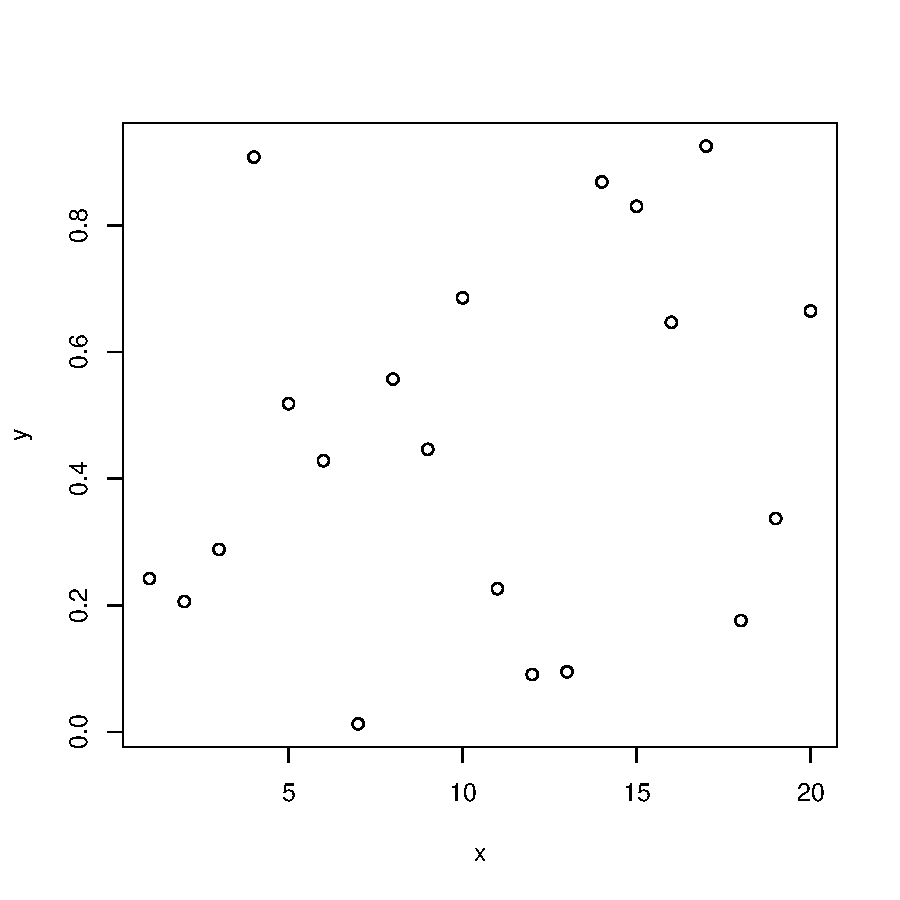
\includegraphics{r-cmd-022}
\caption{Gewöhnlicher Plot mit \lstinline{plot()}}
\end{subfigure}
\begin{subfigure}[b]{0.48\textwidth}
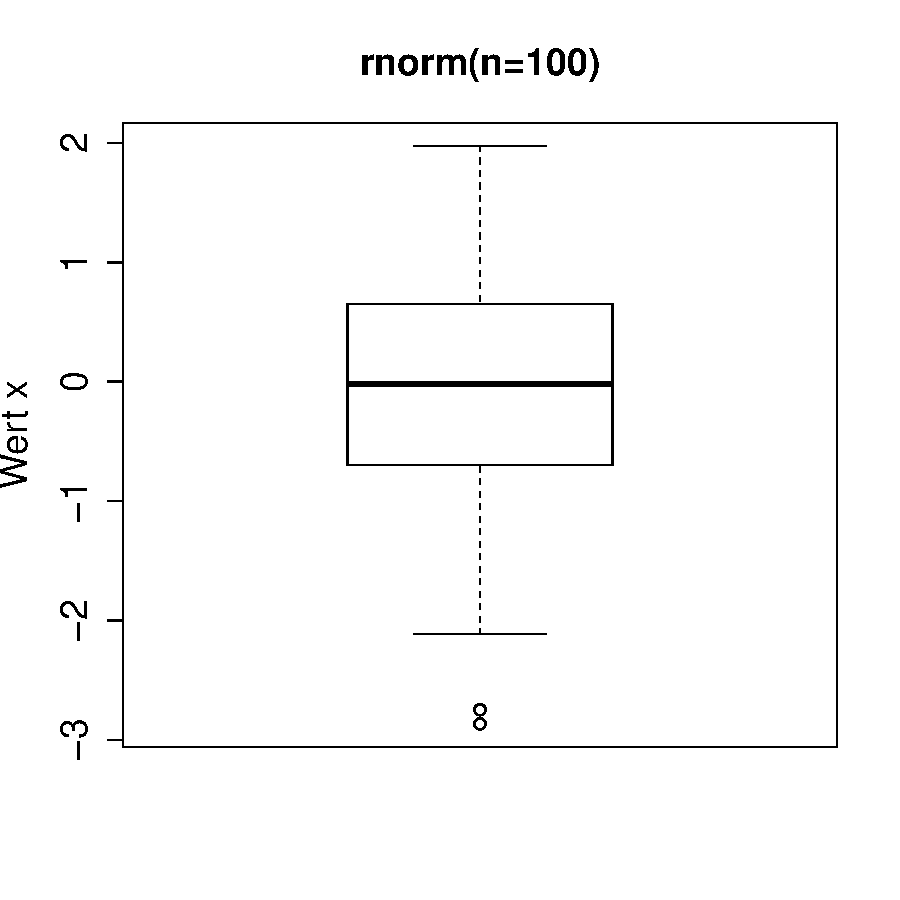
\includegraphics{r-cmd-023}
\caption{Linie mit \lstinline{abline()}}
\end{subfigure}

\begin{subfigure}[b]{0.48\textwidth}
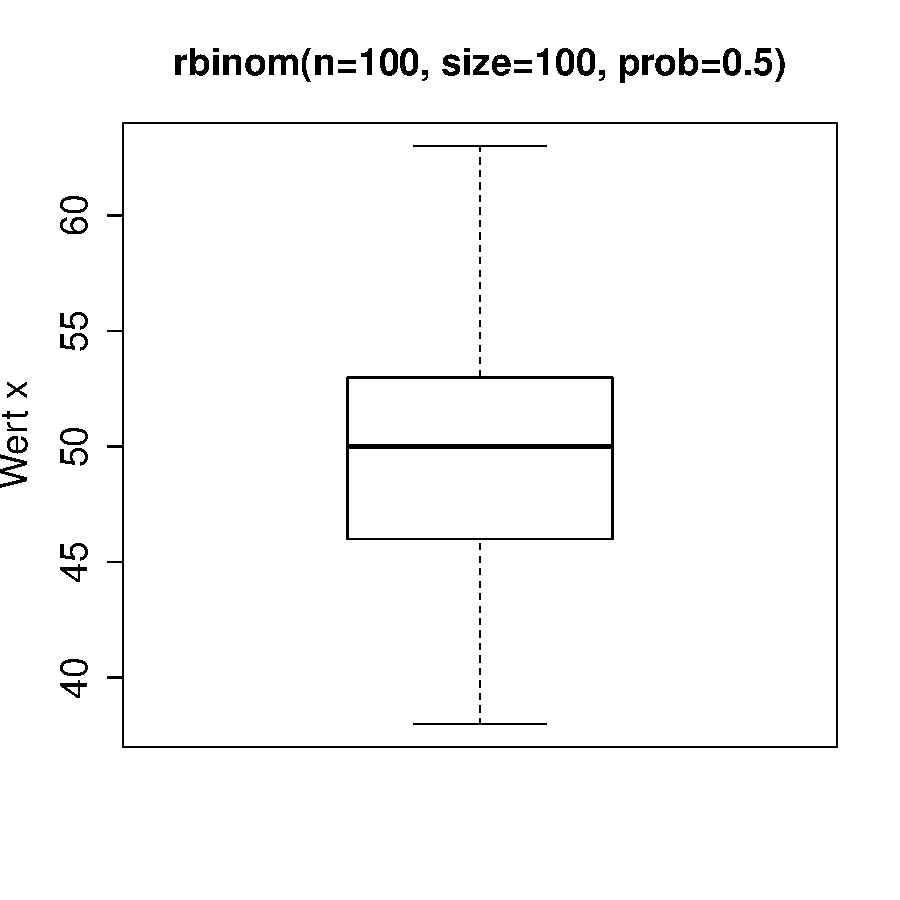
\includegraphics{r-cmd-024}
\caption{Segmente mit \lstinline{segments()}}
\end{subfigure}
\begin{subfigure}[b]{0.48\textwidth}
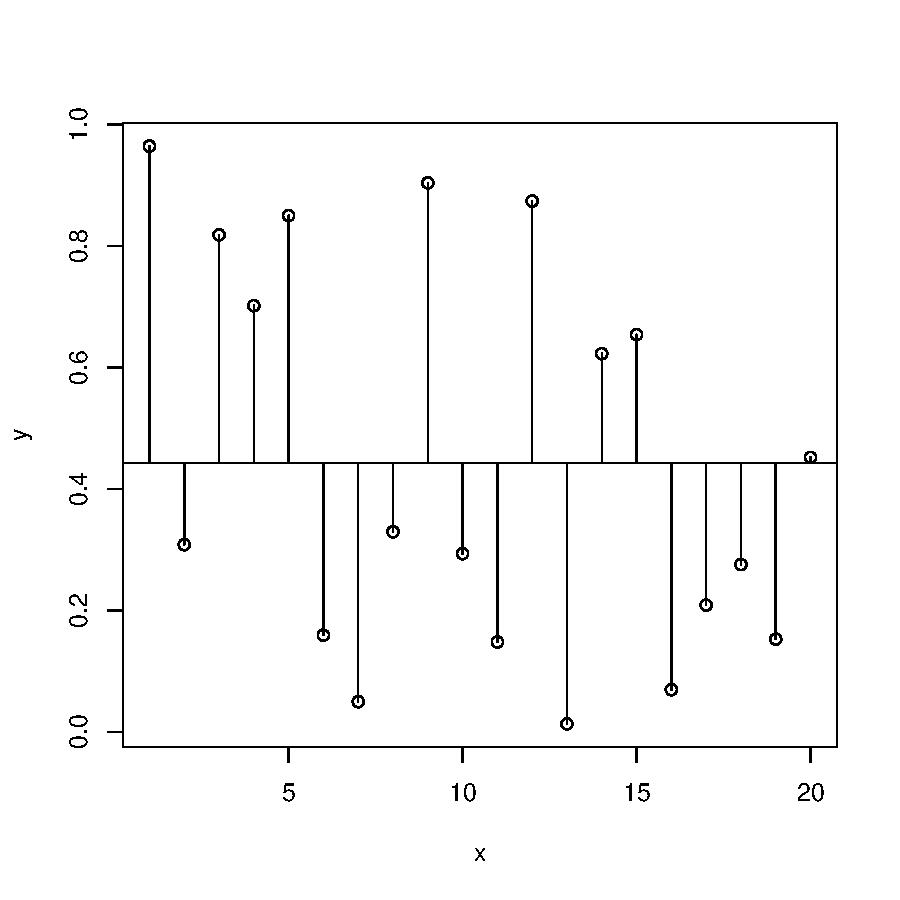
\includegraphics{r-cmd-025}
\caption{Flächen mit \lstinline{rect()}}
\end{subfigure}

\end{figure}

\clearpage

\subsection{Boxplot}
Ein Boxplot zeigt sehr viele Informationen zur Statistik einer 
Datenreihe in einem Plot auf. Insbesondere sind dies
\begin{itemize}
	\item extrem \emph{grosse} Beobachtungen
	\item die grösste \emph{normale} Beobachtung
	\item oberes Quartil ($75$\% Quantil)
	\item Median ($50$\% Quantil)
	\item unteres Quartil ($25$\% Quantil)
	\item die kleinste \emph{normale} Beobachtung
	\item extrem \emph{kleine} Beobachtungen
\end{itemize}
Die Abbildung \ref{fig:boxplot} zeigt einen Boxplot welches alle
oben genannten Merkmale gut sichtbat enthält.

\begin{figure}[h!]
	\centering
	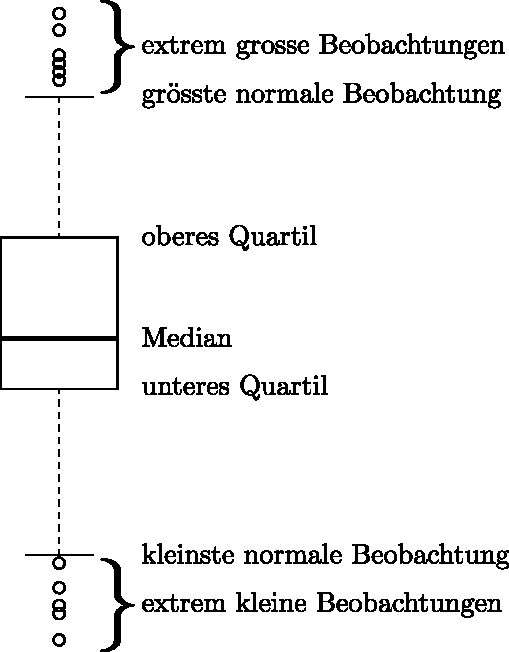
\includegraphics[width=0.5\textwidth]{boxplot.pdf}
	\caption{Analyse eines Boxplots}
	\label{fig:boxplot}
\end{figure}

\noindent
Mit solch einem Plot lässt sich die Verteilung einer Datenreihe sehr
schnell graphisch erfassen ohne dabei zu rechnen oder etwas 
interpretieren zu müssen. Jede Verteilung hat ihre spezielle 
Charakteristik die sich im Boxplot erkennen lässt.
\begin{itemize}
	\item Die uniforme Verteilung hat in etwa gleich grosse Bereiche
		der Quartile, ist somit symetrisch und geht über den 
		ganzen Bereich und hat somit keine Ausreisser 
		(Extremweerte).
	\item Die binomiale Verteilung hat enger beieinander liegende
		$25$\% Quantile und kann Ausreisser haben.
	\item Die normale Verteilung ist der binomialen sehr ähnlich.
	\item Exponentiale Verteilungen haben unsymetrische Quantile
		und grundsätzlich Ausreisser.
\end{itemize}





\begin{figure}[h!]
\centering
\begin{subfigure}[b]{0.48\textwidth}
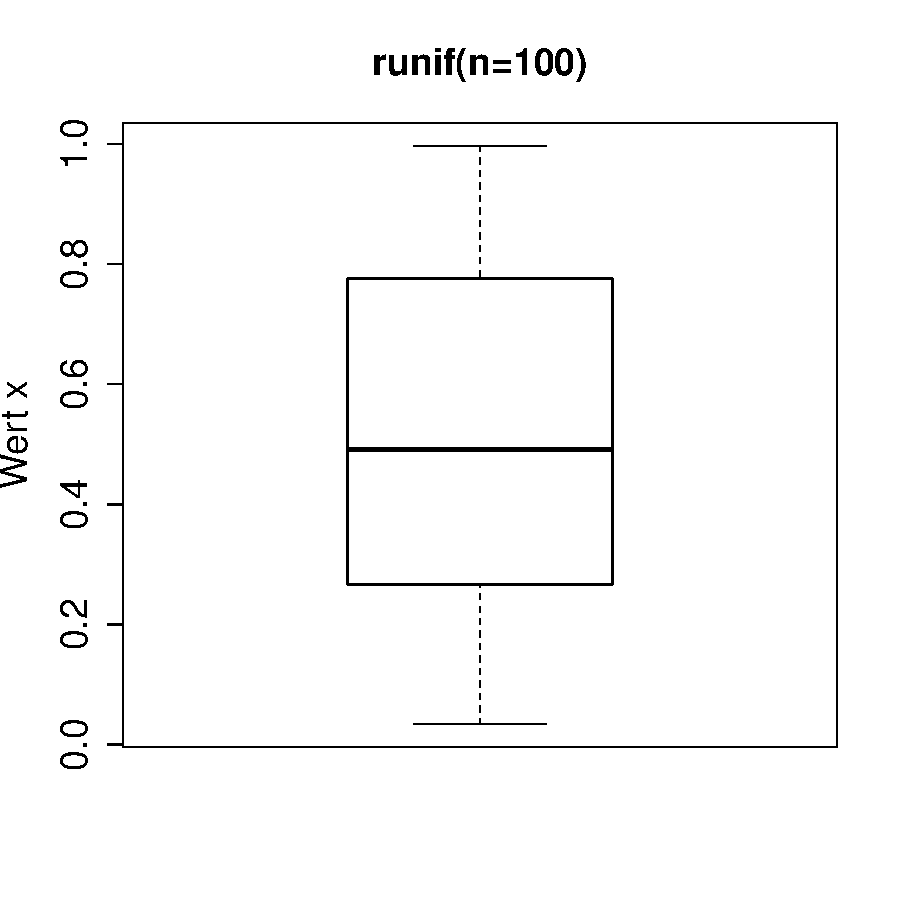
\includegraphics{r-cmd-030}
\caption{Uniforme Verteilung}
\end{subfigure}
\begin{subfigure}[b]{0.48\textwidth}
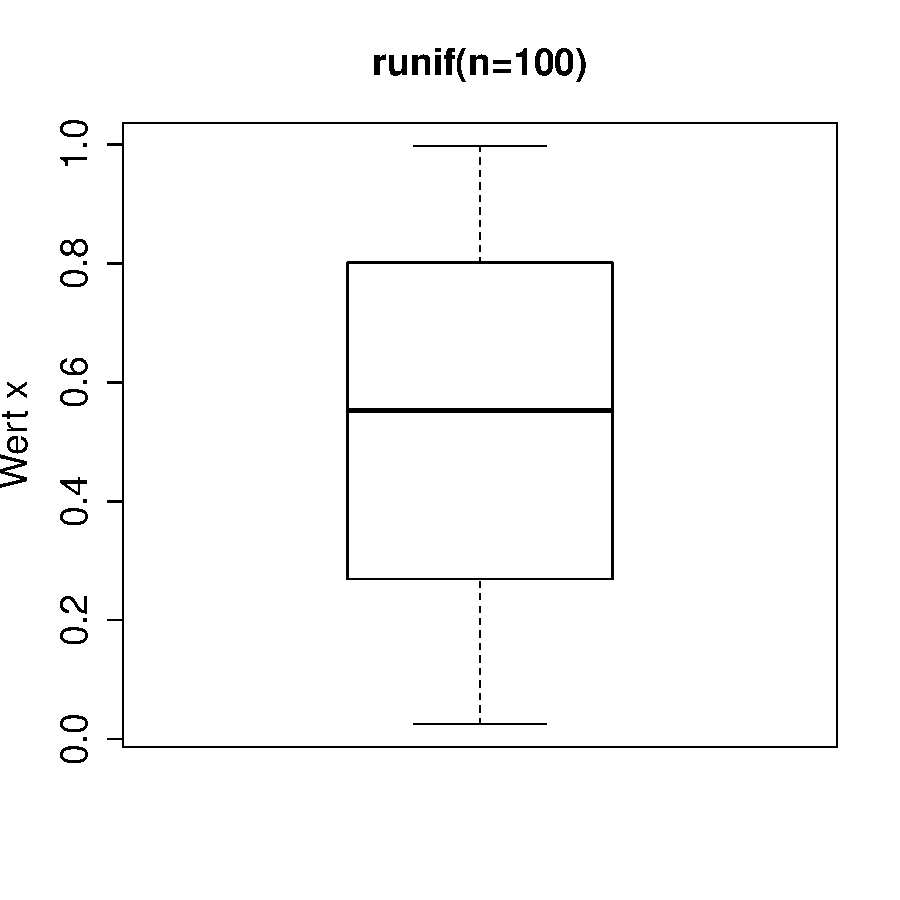
\includegraphics{r-cmd-031}
\caption{Binomiale Verteilung}
\end{subfigure}

\begin{subfigure}[b]{0.48\textwidth}
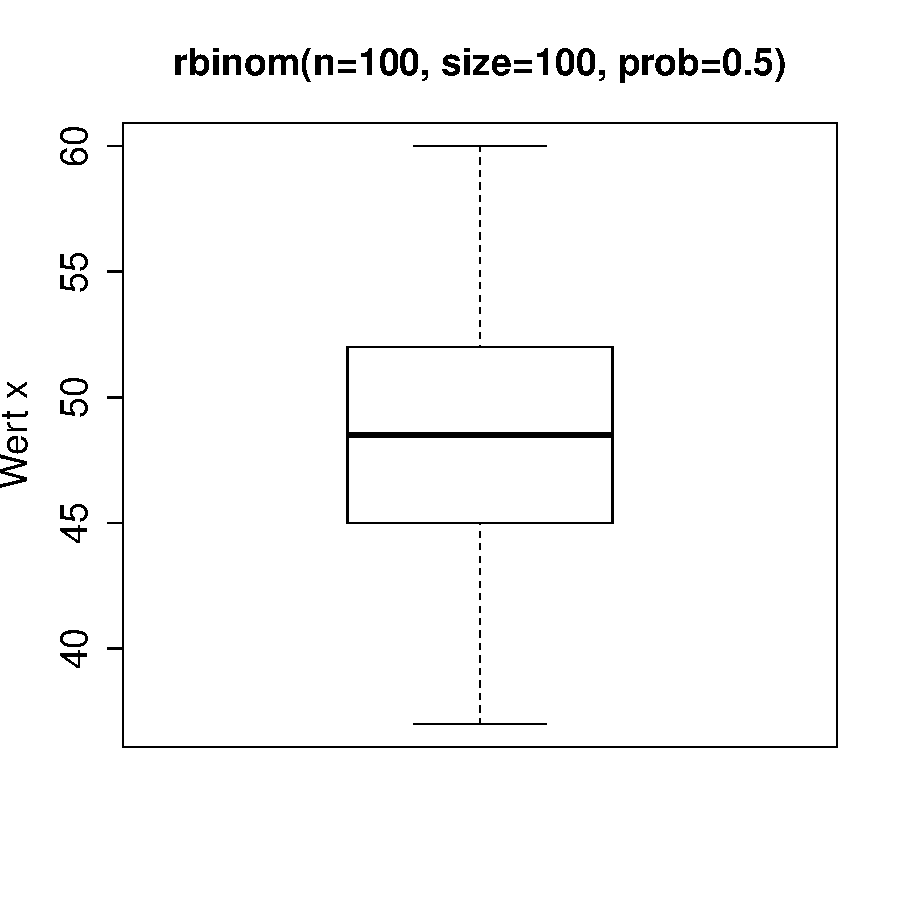
\includegraphics{r-cmd-032}
\caption{Normale Verteilung}
\end{subfigure}
\begin{subfigure}[b]{0.48\textwidth}
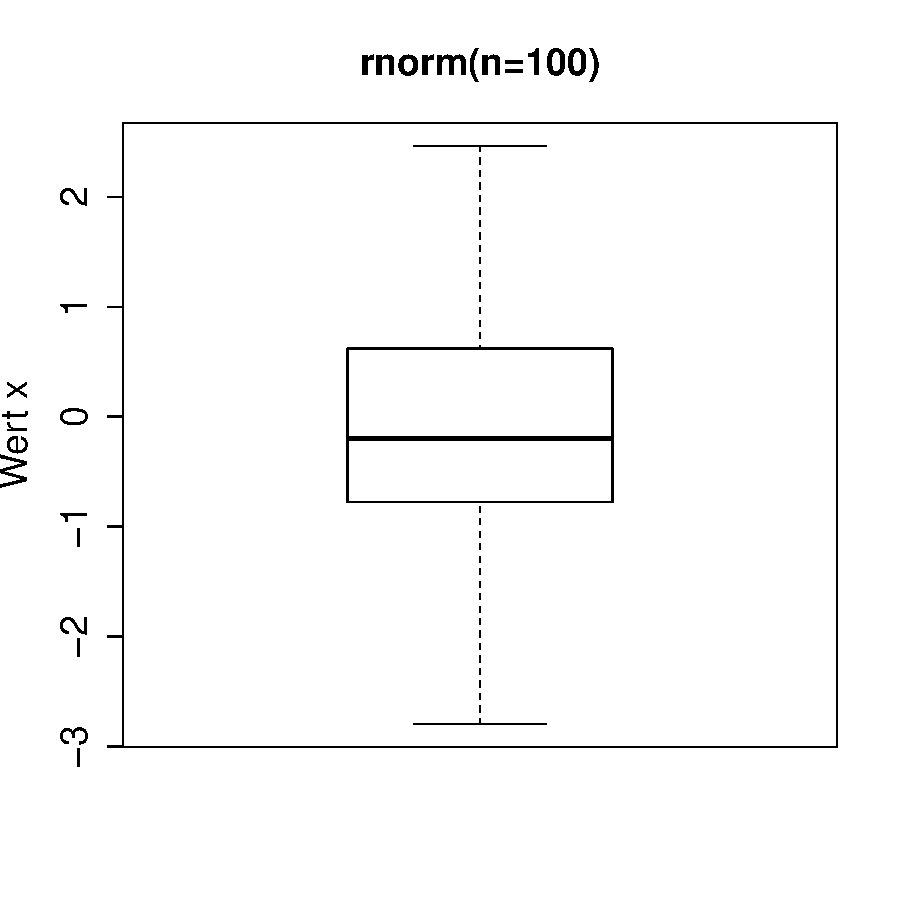
\includegraphics{r-cmd-033}
\caption{Exponential Verteilung}
\end{subfigure}
\caption{Boxplots verschiedener Verteilungen}
\end{figure}

\clearpage
\section{Daten benutzen}
\lstinline{R} kennt neben einfachen Variablen, Vektoren und Matrizen
auch sog. \emph{Data Frames}. Diese sind den Matrizen ähnlich mit dem
Unterschied, dass man in einem solchen Data Frame verschiedene Typen
ablegen kann (Zahlen, Buchstaben etc.) während Matrizen nur
numerische Inhalte haben können.

\subsection{Daten zusammenstellen}
Ein Data Frame kann mit der Funktion \lstinline{data.frame()} erstellt
werden.

\begin{Schunk}
\begin{Sinput}
> a <- c(1.67, 1.82, 1.76, 1.94)
> b <- c("m", "f", "f", "m")
> c <- c(12, 19, 23, 17)
> team <- data.frame(a, b, c)
> team
\end{Sinput}
\begin{Soutput}
     a b  c
1 1.67 m 12
2 1.82 f 19
3 1.76 f 23
4 1.94 m 17
\end{Soutput}
\end{Schunk}

\subsubsection{Daten benennen}
Möchte man das Data Frame um sog. \emph{header} erweitern,
so kann man die Funktion \lstinline{colnames()} nutuzen

\begin{Schunk}
\begin{Sinput}
> a <- c(1.67, 1.82, 1.76, 1.94)
> b <- c("m", "f", "f", "m")
> c <- c(12, 19, 23, 17)
> team <- data.frame(a, b, c)
> colnames(team) <- c("Height", "Sex", "Age")
> team
\end{Sinput}
\begin{Soutput}
  Height Sex Age
1   1.67   m  12
2   1.82   f  19
3   1.76   f  23
4   1.94   m  17
\end{Soutput}
\end{Schunk}

\noindent
Es ist aber auch möglich das komplette Data Frame mit Labels
zu versehen mit der Funktion \lstinline{dimnames()}. Hierzu
muss aber eine \emph{list} als Parameter übergeben werden
welche je einen Vektor für Spalten und Reihen hat.

\begin{Schunk}
\begin{Sinput}
> a <- c(1.67, 1.82, 1.76, 1.94)
> b <- c("m", "f", "f", "m")
> c <- c(12, 19, 23, 17)
> team <- data.frame(a, b, c)
> columns <- c("Babbage", "Lovelace", 
+ 	     "Noether", "Shannon")
> rows <- c("Height", "Sex", "Age")
> dimnames(team) <- list(columns, rows)
> team
\end{Sinput}
\begin{Soutput}
         Height Sex Age
Babbage    1.67   m  12
Lovelace   1.82   f  19
Noether    1.76   f  23
Shannon    1.94   m  17
\end{Soutput}
\end{Schunk}

\subsubsection{Daten faktorisieren}
Bei der Erstellung von Data Frames ist es sinnvoll für typisierte
Daten die Funktion \lstinline{factor()} zu nutzen, denn diese 
ermöglicht es Datenreihen zu \emph{faktorisieren}. 

Beispielsweise hat man einen Datensatz bei dem das Geschlecht 
verzeichnet ist. Das Geschlecht kann zwei Werte annehmen, sog. 
\emph{Levels}.

\begin{Schunk}
\begin{Sinput}
> a <- c(1.67, 1.82, 1.76, 1.94, 1.86, 1.78)
> b <- factor(c("m", "f", "f", "m", "f", "m"))
> c <- c(12, 19, 23, 17, 20, 24)
> team <- data.frame(a, b, c)
> colnames(team) <- c("Alter", "Hoehe", "Geschlecht")
> team
\end{Sinput}
\begin{Soutput}
  Alter Hoehe Geschlecht
1  1.67     m         12
2  1.82     f         19
3  1.76     f         23
4  1.94     m         17
5  1.86     f         20
6  1.78     m         24
\end{Soutput}
\begin{Sinput}
> b
\end{Sinput}
\begin{Soutput}
[1] m f f m f m
Levels: f m
\end{Soutput}
\end{Schunk}

\subsection{Daten von URL einbinden}
Steht ein Datensatz als Tabelle auf einer Webseite zur Verfügung,
so kann man diese mit der Funktion \lstinline{read.table()} einbinden.

Hierbei gilt es zu beachten, dass die Formatierung berücksichtigt
werden muss. Bispielsweise ob die Daten kommasepariert 
(\lstinline{sep}) sind oder ob die Daten je einen Titel 
(\lstinline{header}) haben.

\begin{Schunk}
\begin{Sinput}
> url <- "http://data.princeton.edu/wws509/datasets/effort.dat"
> data <- read.table(url, header=TRUE)
> data
\end{Sinput}
\begin{Soutput}
               setting effort change
Bolivia             46      0      1
Brazil              74      0     10
Chile               89     16     29
Colombia            77     16     25
CostaRica           84     21     29
Cuba                89     15     40
DominicanRep        68     14     21
Ecuador             70      6      0
ElSalvador          60     13     13
Guatemala           55      9      4
Haiti               35      3      0
Honduras            51      7      7
Jamaica             87     23     21
Mexico              83      4      9
Nicaragua           68      0      7
Panama              84     19     22
Paraguay            74      3      6
Peru                73      0      2
TrinidadTobago      84     15     29
Venezuela           91      7     11
\end{Soutput}
\end{Schunk}

\subsection{Daten verarbeiten}
Um Daten eines Data Frame zu bearbeiten kann genau wie bei Matrizen
vorgegenagen werden. Für die effiziente Bearbeitung ganzer Reihen
oder Spalten gibt es neben den iterativen Methoden mit Schlaufen noch
den funktionalen Ansatz mittels der \lstinline{apply()} Funktionen
von denen es drei verschiedene gibt.

\begin{itemize}
	\item \lstinline{apply()}
	\item \lstinline{lapply()}
	\item \lstinline{sapply()}
\end{itemize}

Allen gemeinsam ist, dass diese eben funktional sind, d.h. man
kann nur Funktionen auf etwas anwenden. Beispielsweise um Datenwerte
um eine Dekade zu vergrössern müsste man eine Funktion definieren
die dies bewerkstelligt.

\begin{Schunk}
\begin{Sinput}
> a <- 13.5
> decadeUp <- function(x) {x*10}
> b <- decadeUp(a)
> b
\end{Sinput}
\begin{Soutput}
[1] 135
\end{Soutput}
\end{Schunk}

Im Folgenden sind die einzelnen Funktionen nochmals mit kurzen 
Beispielen erläutert.

\subsubsection{\lstinline{apply()}}
Die Funktion \lstinline{apply()} ermöglicht es, eine Funktion auf
alle Elemente eines Arrays oder eines Data Frames anzuwenden.

\begin{Schunk}
\begin{Sinput}
> age <- c(11, 24, 33, 17)
> weight <- c(53, 79, 68, 86)
> height <- c(1.39, 1.82, 1.67, 1.87)
> team <- data.frame(age, weight, height)
> team
\end{Sinput}
\begin{Soutput}
  age weight height
1  11     53   1.39
2  24     79   1.82
3  33     68   1.67
4  17     86   1.87
\end{Soutput}
\begin{Sinput}
> # die Hoehe vom Meter in Centimeter wandeln
> toCentimeter <- function(x) {x*100}
> team[3] <- apply(team[3], MARGIN=2, FUN=toCentimeter)
> team
\end{Sinput}
\begin{Soutput}
  age weight height
1  11     53    139
2  24     79    182
3  33     68    167
4  17     86    187
\end{Soutput}
\end{Schunk}

\subsubsection{\lstinline{lapply()}}
\subsubsection{\lstinline{sapply()}}
